\part{Apprentissage}
\pagebreak

\chapter{Approche d'apprentissage par la logique}
Une approche simple concernant l'apprentissage de problèmes dont le domaine de sortie est boolean
serait de passer par la logique classique pour pouvoir simplifier la compréhension du problème.\\
\pagebreak
\section{Espace de Version}
Pour un problème suivant:

$\begin{tabular}{cccc|c}
\hline
A & B & C & D & accaptable? \\
\hline
1 & 1 & 1 & 0 & oui\\
1 & 1 & 0 & 1 & oui\\
0 & 1 & 1 & 1 & non\\
\hline
\end{tabular}$

\ \\
D'où il suffirait d'une fonction donnant dans le domaine Boolean, associer un algorithme de classification simple:\\
\ \\
\vspace{1cm}
\scalebox{0.7}{
\begin{tikzpicture}
  \begin{axis} [
      xlabel     = X, % label x axis
      ylabel     = Y, % label y axis
      axis lines = left, %set the position of the axes
      clip       = false, 
      xmin       = 0,
      ymin       = 0,
    ]
    \addplot [color=black] coordinates { (0,0)(5,5) };
    \addplot [only marks, mark=*, color=blue] coordinates {(1,4)(3,3.5) };
    \addplot [only marks, mark=*, color=red] coordinates {(4,2) };
  \end{axis}
\end{tikzpicture}
}

\vspace{1cm}

Ayant comme points de couleurs $\crouge{Rouge}$ les points donnant la valeur de vérité False et les points de couleurs $\cblue{Blue}$ les point donnant la valeur de vérité True.\\
Mais ce ne serait pas donner un gros mode de résolution à un problème qui peut être simplifié?\\
\\
Pour les cas suivants:
\begin{description}
\item[-] Faciliter la compréhension du problème
\item[-] Comprendre pourquoi une décision donné pour une entrée
\end{description}
\pagebreak

\subsection{convergence des données}

Dans le tableau d'acceptation on peut transformé la règle 3 en son dual via la Lois de De Morgan:\\

\begin{multicols}{2}
[Et via un treillis de donnée pour chaque entré positif on peut compter le nombre d'occurrence de motif en faveur de l'acceptation de la ligne:]
\scalebox{0.3}{
\begin{tikzpicture}[->,>=stealth',shorten >=1pt,auto,node distance=2.8cm,
                    semithick]
  \tikzstyle{every state}=[fill=white,draw=none,text=black]

  \node[state]         (Z)                    {$\{\}$};
  \node[state]         (B) [below left  of=Z] {$B$};
  \node[state]         (A) [left  of=B]       {$A$};
  \node[state]         (C) [below right of=Z] {$C$};
  \node[state]         (D) [right of=C]       {$D$};
  \node[state]		   (AC) [below  of=A]     {$AC$};
  \node[state]		   (AB) [left of=AC]      {$AB$};
  \node[state]		   (AD) [right of=AC]     {$AD$};
  \node[state]         (BC) [right of=AD]     {$BC$};
  \node[state]		   (BD) [right of=BC]	  {$BD$};
  \node[state]		   (CD) [right of=BD] 	  {$CD$};
  \node[state]		   (ABD) [below of=AD]    {$ABD$};
  \node[state] 		   (ABC) [left of=ABD]    {$ABC$};
  \node[state]		   (ACD) [right of=ABD]   {$ACD$};
  \node[state]		   (BCD) [right of=ACD]   {$BCD$};
  \node[state]	       (ABCD) [below of=ABD]  {$ABCD$};
  

  \path (Z) edge              node {} (A)
            edge              node {} (B)
            edge			  node {} (C)
            edge  			  node {} (D)
        (A) edge			  node {} (AB)
        	edge			  node {} (AC)
        	edge			  node {} (AD)
        (B) edge			  node {} (AB)
        	edge			  node {} (BC)
        	edge 			  node {} (BD)
        (C) edge 			  node {} (AC)
        	edge			  node {} (BC)
        	edge 			  node {} (CD)
        (D) edge 			  node {} (AD)
        	edge 			  node {} (BD)
        	edge 			  node {} (CD)
        (AB) edge 			  node {} (ABC)
        	edge 			  node {} (ABD)
        (AC) edge			  node {} (ABC)
        	edge 			  node {} (ACD)
        (AD) edge 			  node {} (ABD)
        	edge			  node {} (ACD)
        (BC) edge			  node {} (ABC)
        	edge  			  node {} (BCD)
        (BD) edge			  node {} (ABD)
        	edge 			  node {} (BCD)
        (CD) edge 			  node {} (ACD)
        	edge			  node {} (BCD)
        (ABC) edge 			  node {} (ABCD)
        (ACD) edge 			  node {} (ABCD)
        (ABD) edge 			  node {} (ABCD)
        (BCD) edge 			  node {} (ABCD);
\end{tikzpicture}
}
$\begin{tabular}{cccc|c}
\hline
A & B & C & D & accaptable? \\
\hline
1 & 1 & 1 & 0 & oui\\
1 & 1 & 0 & 1 & oui\\
1 & 0 & 0 & 0 & oui\\
\hline
\end{tabular}$
\end{multicols}
\ \\

\begin{multicols}{2}
[]
\scalebox{0.4}{
\begin{tikzpicture}[->,>=stealth',shorten >=1pt,auto,node distance=2.8cm,
                    semithick]
  \tikzstyle{every state}=[fill=white,draw=none,text=black]

  \node[state]         (Z)                    {$\{\}$};
  \node[state]         (B) [below  of=Z]      {$B$};
  \node[state]         (A) [left  of=B]       {$A$};
  \node[state]         (C) [right of=B]       {$C$};
  \node[state]		   (AB) [below of=A]      {$AB$};
  \node[state]		   (AC) [right of=AB]     {$AC$};
  \node[state]         (BC) [right of=AC]     {$BC$};
  \node[state] 		   (ABC) [below of=AC]    {$ABC$};
  

  \path (Z) edge              node {} (A)
            edge              node {} (B)
            edge			  node {} (C)
        (A) edge			  node {} (AB)
        	edge			  node {} (AC)
        (B) edge			  node {} (AB)
        	edge			  node {} (BC)
        (C) edge 			  node {} (AC)
        	edge			  node {} (BC)
        (AB) edge 			  node {} (ABC)
        (AC) edge			  node {} (ABC)
        (BC) edge			  node {} (ABC);
\end{tikzpicture}
}
$\begin{tabular}{cccc|c}
\hline
A & B & C & D & accaptable? \\
\hline
\crouge{1} & \crouge{1} & \crouge{1} & \crouge{0} & \crouge{oui}\\
1 & 1 & 0 & 1 & oui\\
1 & 0 & 0 & 0 & oui\\
\hline
\end{tabular}$
\end{multicols}
\pagebreak

\begin{multicols}{2}
[]
\scalebox{0.4}{
\begin{tikzpicture}[->,>=stealth',shorten >=1pt,auto,node distance=2.8cm,
                    semithick]
  \tikzstyle{every state}=[fill=white,draw=none,text=black]

  \node[state]         (Z)                    {$\{\}$};
  \node[state]         (B) [below  of=Z]      {$B$};
  \node[state]         (A) [left  of=B]       {$A$};
  \node[state]		   (AB) [below of=A]      {$AB$};
  

  \path (Z) edge              node {} (A)
            edge              node {} (B)
        (A) edge			  node {} (AB)
        (B) edge			  node {} (AB);
\end{tikzpicture}
}
$\begin{tabular}{cccc|c}
\hline
A & B & C & D & accaptable? \\
\hline
1 & 1 & 1 & 0 & oui\\
\crouge{1} & \crouge{1} & \crouge{0} & \crouge{1} & \crouge{oui}\\
1 & 0 & 0 & 0 & oui\\
\hline
\end{tabular}$
\end{multicols}

\begin{multicols}{2}
[]
\scalebox{0.4}{
\begin{tikzpicture}[->,>=stealth',shorten >=1pt,auto,node distance=2.8cm,
                    semithick]
  \tikzstyle{every state}=[fill=white,draw=none,text=black]

  \node[state]         (Z)                    {$\{\}$};
  \node[state]         (A) [left  of=B]       {$A$};
  

  \path (Z) edge              node {} (A);
\end{tikzpicture}
}
$\begin{tabular}{cccc|c}
\hline
A & B & C & D & accaptable? \\
\hline
1 & 1 & 1 & 0 & oui\\
1 & 1 & 0 & 1 & oui\\
\crouge{1} & \crouge{0} & \crouge{0} & \crouge{0} & \crouge{oui}\\
\hline
\end{tabular}$
\end{multicols}

\ \\
Par itération et réduction du treillis on sait que $A$ et un attribut très discriminant, qui fait revenir le problème à seulement la valeur de $A$.\\

\pagebreak
\chapter{Apprentissage statistique}

Dans ce chapitre nous nous intéressons à des fonctions $h \in H$ à qui pour une liste $X$ à $d$ dimension de domaine réelle associe un label $y$ dans le domaine $[-1,+1]$. Un $x \in X$ peut être une couleur, un réelle, une chose négatif ou encore une mesure quelconque.
\pagebreak

\section{Classification binaire réalisable}

Chaque entrée $x \in X$ est tirée aléatoirement et indépendamment selon une distribution de probabilité $d$ qui est fixée mais inconnue de l'apprenant.
\\
Chaque sortie $y \in Y$ est calculé via la fonction cible $h* \in H$ qui est inconnue de l'apprenant.

\subsection{Erreur de généralisation et d'entrainement}

La performance d'une hypothèse $h \in H$ est calculé par le nombre d'erreurs que la fonction peut commettre en probabilité selon $d$:
\begin{description}
\item[] $l_d(h)$ = $P_{x~d}[h(x) \neq h*(x)]$
\end{description}

En pratique, l'apprenant n'a accès qu'a une petite partit nommé $S \in X$ (qui peut contenir des doublons) dont les éléments dont générés aléatoirement via $d$, Le risque empirique de $h$ par rapport à $S$ est donné par :
\begin{description}
\item[] $l_s(h)$ = $\frac{1}{|S|} |\{x \in S : h(x) \neq h*(x)\}|$
\end{description}
Le nombre d'erreur moyen que fait $h$ sur $S$\\

\subsection{Processus d'apprentissage}

Le processus d'apprentissage n'est pas si différent que dans la première partie du Memo:\\

Soit une distribution $d$, chaque requêtes vers $d$ va choisir un échantillons aléatoirement pour crée un ensemble $S$ qui va servir à faire apprendre $h$ lors de la phase d'apprentissage, tester lors de la phase de teste et retenir les erreur vies les fonction d'analyse.\\

\subsection{Incertitude de l'apprentissage}

Il existe deux mesures de l'incertitude en apprentissage statistique
\begin{description}
\item[] Paramètre de confiance qui donne la qualité de l'échantillonnage
\item[] Paramètre d'erreur qui donne un indice sur les bonnes prédictions futures
\end{description}

\subsection{Modèle PAC réalisable}
Une classe d(hypothèses $H$ est dite PCA (probability approximately correct) s'il existe une fonction $\{0,1\}^2 \rightarrow \{0,1,2.....\}$ telle que pour toute paire ($\phi$(confiance),$\psi$(erreur)) pour toute distribution $d$ sur $X$ et toute fonction cible $h* \in H$:
\begin{description}
\item[] Après avoir observé un échantillon $S$ de $X$ tiré aléatoirement selon $d$, et de taille au moins $m(\phi,\psi)$.
\item[] L'apprenant retourne une hypothèse $h \in H$, telle qu'avec une probabilité au moins $1 - \phi$, l'erreur de génération $l_d(h)$ est d'au plus $\psi$.
\end{description}

\section{Classes d'hypothèses finies}

Supposons $X$ = $[0,1]^d$

\begin{description}
\item[] Toutes fonction $h: [0,1]^d \rightarrow [0,1]$ est appelée fonction booléenne.
\item[] Une classe d'hypothèses booléennes est un sous ensemble $H$ de $[[0,1]^d \rightarrow [0,1]]$.
\end{description}

\subsection{Minimisation des erreurs empirique}
Le principe est de trouver dans $H$ l'hypothèse qui fait le moins d'erreurs sur l'échantillon $S$:
\formula{$h_S \in argmin L_S(h), h \in H$}


\subsection{Théorème de PAC des classes finies}
Toutes classe d'hypothèse $H$ finie est PAC-apprenable avec une complexité d'échantillonnage
\formula{$m(\phi,\psi) \leq \frac{ln(|H|/\phi)}{\psi}$}

\pagebreak
\section{Apprentissage agnostique}
\subsection{Principe de minimisation de risque empirique}

\section{VC Dimension}
\subsection{Fonctions linéaires}
\subsection{Fonctions de croissance et VC-Dimension}
\subsection{Théorème fondamental de l'apprentissage statistique}

Une version Qualitative:
\begin{description}
\item[] Soit $H$ une classe de fonctions $X$ dans $\{0,1\}$ mesurée selon la fonction de perte discrète (nombre d'erreurs), Alors les propriétés suivantes sont équivalentes:
\end{description}
\formula{$H$ est agnostiquement PAX apprenable}
\formula{$H$ a la propriété de convergence uniforme}
\formula{$H$ a une VC-dimension finie}

\ \\
Une version Quantitative:
\begin{description}
\item[] Soit $H$ une classe de fonctions de $X$ dans $\{0,1\}$, mesurée selon la fonction de perte discrète (nombre d'erreurs). Supposons que $VCdim(H) = D < \infty$. Alors il existe une constance $C$ telle que $H$ est agnostiquement PAC apprennable avec une complexité d'échantilonage d'au plus:
\end{description}
\formula{$m(\alpha, \epsilon) \leq C (\frac{D+ln(\frac{1}{\alpha}}{\epsilon^2})$}

\subsection{VC-Dimensions Utiles}

\pagebreak
\chapter{Apprentissage Online}

L'apprentissage online est un jeu à somme nulle répétitif à deux joueur (théorème minmax ou équilibre de Nash), les joueurs sont l'environnement et le joueur.\\
L'apprenant reçoit une observation de l'environnement et donne une prédiction, et l'environnement va donner la vérification sur la prédiction.\\

\pagebreak
\section{Analyse convexe}
\subsection{Combinaison convexe}

Une forme convexe est une forme pour qui n'importe quel droite dont les 2 points font partie de la forme est dans la forme.\\

\begin{center}
\begin{tikzpicture}[scale=2]
    \matrix[nodes={draw, ultra thick, fill=blue!20},
        row sep=0.3cm,column sep=0.5cm] {

    \node[ellipse] {$Convexe$};&
    \node[star,star points=5, scale=0.5] {$Non\ convexe$};\\
    };
\end{tikzpicture}
\end{center}

\subsection{Enveloppe convexe}

L'enveloppe convexe d'une forme est la bordure\\
\begin{center}
\begin{tikzpicture}[scale=2]
    \matrix[nodes={draw, ultra thick, fill=white},
        row sep=0.3cm,column sep=0.5cm] {

    \node[ellipse] {$Convexe$};\\
    };
\end{tikzpicture}
\end{center}

Si un espace d'application est convexe alors le problème est polynomial, sinon le problème est NP-complet.\\

\cshape{1}{
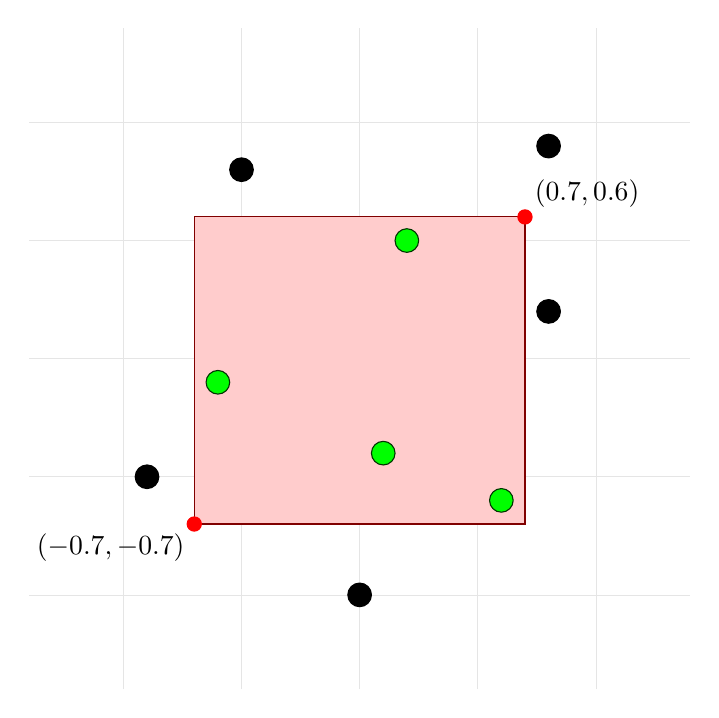
\begin{tikzpicture}[scale=3]
	\draw[step=.5cm,gray!20,very thin] (-1.4,-1.4) grid (1.4,1.4);
	\filldraw[fill=red!20!white, draw=red!50!black] (-0.7,-0.7) rectangle (0.7,0.6);
	
	\foreach \coord in {(-0.5,0.8),(0.8,0.2),(-0.9,-0.5),(0,-1),(0.8,0.9)}{
		\draw[fill=black, draw=black] \coord circle (0.05cm);
	}
	
	\foreach \coord in {(0.2,0.5),(0.1,-0.4),(-0.6,-0.1),(0.6,-0.6)}{
		\draw[fill=green, draw=green!20!black] \coord circle (0.05cm);
	}
	
	\foreach \coord in {(-0.7,-0.7),(0.7,0.6)}{
		\draw[fill=red, draw=red] \coord circle (0.03cm);
	}
	
	\draw (-0.7,-0.7) node[below left] {$(-0.7,-0.7)$};
	\draw (0.7,0.6)   node[above right]{$(0.7,0.6)$};
\end{tikzpicture}
}

Dans cette figure on calcule l'enveloppe en essayant de capturer tout les points vert, un carré de coordonné $(-0.7,-0.7)(0.7,0.6)$ peut largement faire le boulot et résoudre le problème de classification.\\
Le calcule est polynomial (enfin même inférieur) car le calcul de la classification d'un point se fait en un 4 instructions simple:\\
\formula{$classification = \cblue{lambda}\ x,y : -0.7 < x < 0.7\ \cviolet{and}\ -0.7 < y < 0.6$}
Ce raisonnement est valide car il n'y a aucun point noir dans le rectangle rouge.\\

\pagebreak
\subsection{Theoreme de la séparation des hyperplan}

Un hyperplan est un ensemble de points sous la forme (représenté en blue):
\formula{$H = \{x | a^T x = b\}, a \neq 0\ and\ b \in R$}
\ \\
Un hyperespace est un ensemble de points sous le forme (représenté en rouge):
\formula{$H = \{x | a^T x \leq b \}, a \neq 0\ and\ b \in R$}

\cshape{0.8}{
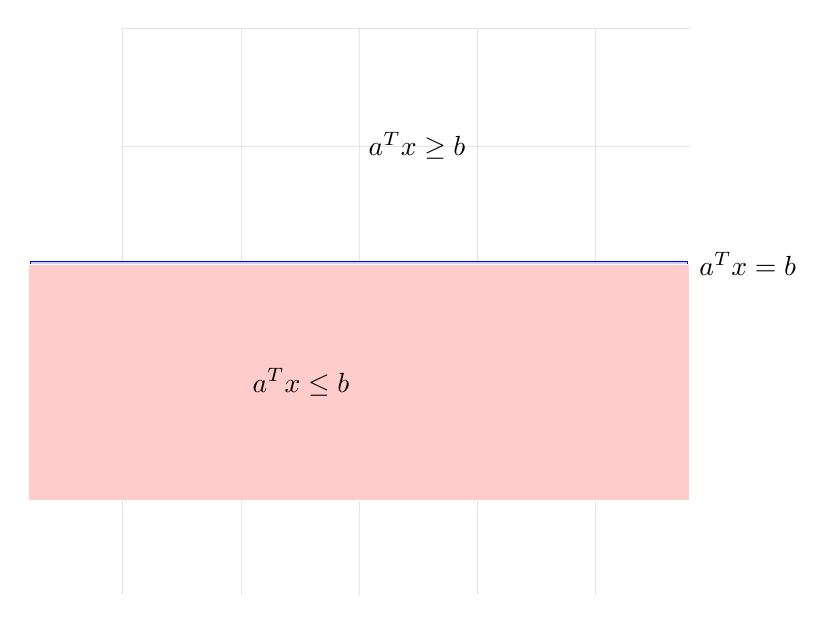
\begin{tikzpicture}[scale=3]
	\draw[step=.5cm,gray!20,very thin] (-1,-1.4) grid (1.4,1);
	\filldraw[fill=blue!20!white, draw=blue!100!black] (-1.39,0.01) rectangle (1.39,-0.01);
	\filldraw[fill=red!20!white, draw=red!0!white] (-1.4,0) rectangle (1.4,-1);
	
	\draw (0,-0.5) node [left] {$\crouge{a^T x \leq b}$};
	\draw (0,0.5)  node [right]{$a^T x \geq b$};
	\draw (1.4,0) node [right] {$\cblue{a^T x = b}$};

\end{tikzpicture}
}
\ \\
Soit $P$ et $N$ deux ensemble de points connexe tel qu'il n'existe aucune intersection, alors il existe une a ($\neq 0$) et un b tel que:
\formula{$a^T x < b \forall x \in P$ and}
\formula{$a^T x \geq b \forall x \in N$}
L'ensemble des $\{x | a^T x = b\}$ est l'hyperplan de séparation de $P$ et $N$ (et aussi une fonction linéaire de classification).

\cshape{0.6}{
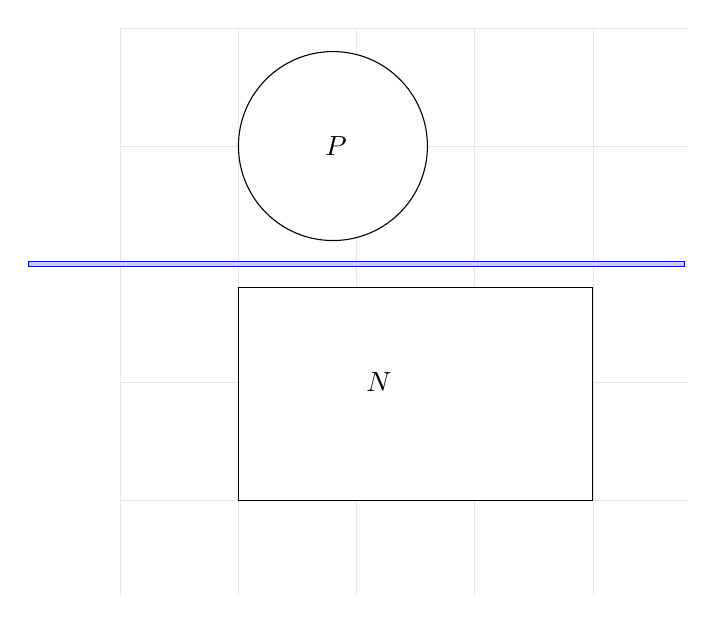
\begin{tikzpicture}[scale=3]
	\draw[step=.5cm,gray!20,very thin] (-1,-1.4) grid (1.4,1);
	\filldraw[fill=white, draw=black] (-0.1,0.5) circle (0.4cm);
	\filldraw[fill=blue!20!white, draw=blue!100!black] (-1.39,0.01) rectangle (1.39,-0.01);
	\filldraw[fill=white, draw=black] (-0.5,-0.1) rectangle (1,-1);
	
	\draw (0,0.5) node [left] {$P$};
	\draw (0,-0.5)  node [right]{$N$};

\end{tikzpicture}
}

\subsection{Fonction convexe et normes}
Une fonction f est dite convexe si son domaine est un ensemble convexe:
\formula{$\forall x,y \in dom(f), \theta \in [0,1]$}
\formula{$f(\theta x + (1-\theta)x) \leq f(x) + (1-\theta) f(x)$}

Autrement dit (via la droite rouge), tout le domaine de la fonction est à l'intérieur de l'ensemble convexe de la fonction parabole:
\begin{multicols}{2}
[]

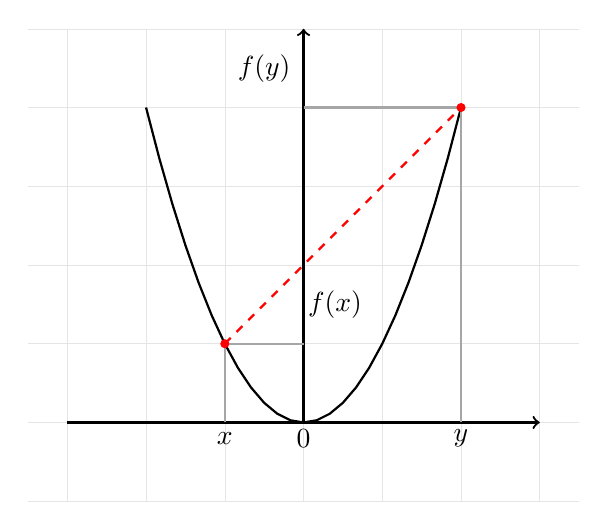
\begin{tikzpicture}
 \draw[help lines, gray!20] (-3.5,-1) grid (3.5,5);

 \draw [->, thick] (-3,0) -- (0,0) -- (3,0);
 \draw [->, thick] (0,0) -- (0,5);
 
 \node at (0,-0.2) {$0$}; 
 \node at (-1,-0.2) {$x$};
 \node at (2,-0.2) {$y$};
 \node at (0.4,1.5) {$f(x)$};
 \node at (-0.5,4.5) {$f(y)$};
 
 \draw [thick, domain=-2:2] plot (\x, {\x*\x});
 \draw [thick, dashed, red] (-1,1) -- (2,4);
 
 \draw [-, thick, gray!70] (-1,0) -- (-1,1);
 \draw [-, thick, gray!70] (-1,1) -- (0,1);
 \draw [-, thick, gray!70] (2,0) --  (2,4);
 \draw [-, thick, gray!70] (2,4) -- (0,4);
 
 \draw [fill, red] (-1,1) circle [radius=0.05];
 \draw [fill, red] (2,4) circle [radius=0.05];
\end{tikzpicture}


\begin{description}
\item[$e^{px}$] est convexe dans R $\forall p \in R$
\item[$|x|^p$]  est convexe dans R si $p \leq 1$
\item[$x log x$]est convexe dans $R^+$ (Entropie)
\item[$||\vec{x}||_p$] Toutes les normes dans $R^n$ sont convexe 
\end{description}
\end{multicols}

La $norme\ 1$ est donné par la somme des coefficient sous forme absolu, on dit aussi le calcule de la distance de Manhattan:
\formula{$||\vec{x}||_1 = |x_1| + ... |x_n|$}

La $norme\ 2$ est obtenu par le produit scalaire, elle est aussi utilisé pour calculer la distance entre 2 points dans un espace vectoriel:
\formula{$||\vec{x}||_2 = \sqrt{|x_1|^2 + ... |x_n|^2}$}

La $norme\ p$ est une généralisation de l'espace de fonction, si on prend $p=2$ on se réduit au produit scalaire:
\formula{$||\vec{x}||_p = (|x_1|^p + ... |x_n|^p)^{\frac{1}{p}}$}

La $norme\ \infty$:
\formula{$||\vec{x}||_{\infty} = max(|x_1|, ... |x_n|)$}

\subsection{Gradient}
Soit $f: R^n \rightarrow R$ et $x$ un point intérieur du domaine de $f$, Si on peut crée une tangente $\frac{\eth f(x)}{\eth x_i}$ (en rouge), on peut dire que $f$ est différentiable (une dérivée existe) passant par $x$:
\cshape{0.7}{
 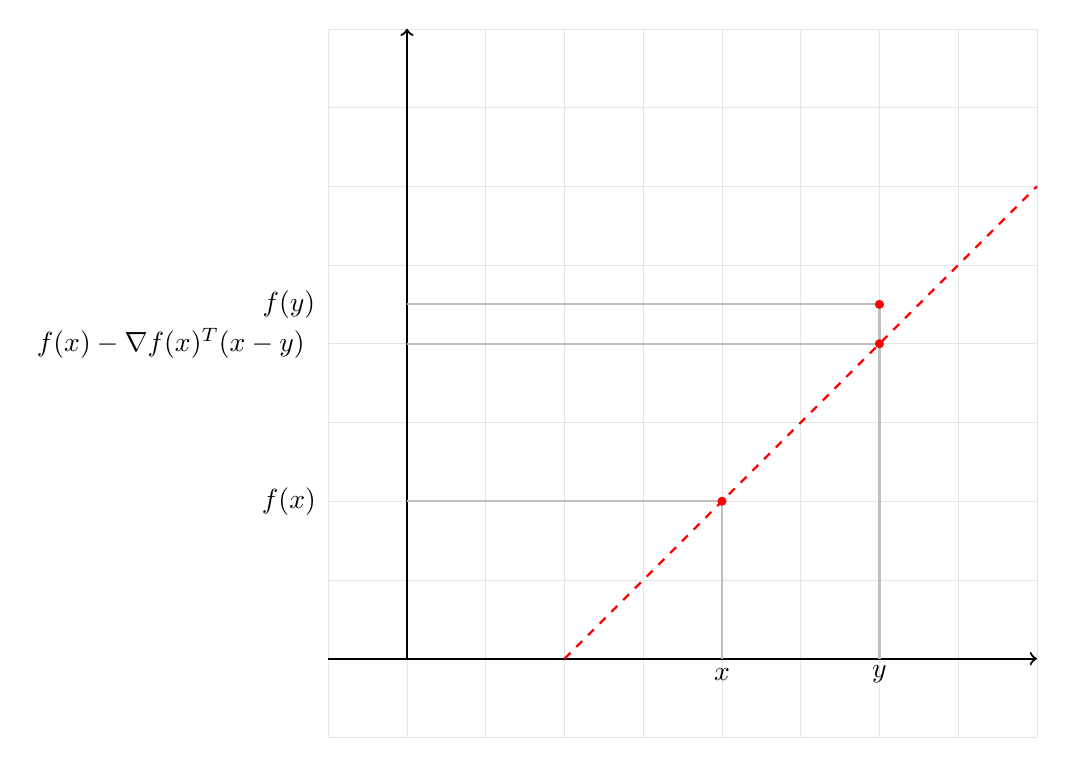
\begin{tikzpicture}
 \draw[help lines, gray!20] (-1,-1) grid (8,8);

 \draw [->, thick] (-1,0) -- (0,0) -- (8,0);
 \draw [->, thick] (0,0) -- (0,8);
 
 \node at (4,-0.2) {$x$}; 
 \node at (6,-0.2) {$y$};
 \node at (-1.5,2)   {$f(x)$};
 \node at (-3,4)   {$f(x)-\nabla f(x)^T(x-y)$};
 \node at (-1.5,4.5) {$f(y)$};
 
 %% \draw [thick, blue, domain=0:3] plot (\x, {\x });
 \draw [thick, dashed, red] (2,0) -- (8,6);
 
 \draw [-, thick, gray!50] (0,2) -- (4,2);
 \draw [-, thick, gray!50] (4,0) -- (4,2);
 \draw [-, thick, gray!50] (0,4) --  (6,4);
 \draw [-, thick, gray!50] (6,0) -- (6,4.5);
 \draw [-, thick, gray!50] (0,4.5) -- (6,4.5);
 
 \draw [fill, red] (4,2) circle [radius=0.05];
 \draw [fill, red] (6,4) circle [radius=0.05];
 \draw [fill, red] (6,4.5) circle [radius=0.05];
\end{tikzpicture}
}

Si $f: R^n \rightarrow R$ est différentiable, alors $f$ est convexe si et seulement si le domaine de $f$ est convexe et $\forall x,y \in f$:
\formula{$f(x) - f(y) \leq \nabla f(x)^T (x-y)$}

\pagebreak
\subsection{Fonction de Perte}

Une fonction de perte est une fonction de $R$ x $R \rightarrow R^+$ tel que pour un couple $(y',y)$ d'une prédiction et d'une vrai réponse, comparer les deux valeurs et retourne si elle sont égal.
\formula{$f(y',y) \rightarrow y' == y$}

\cshape{1}{
 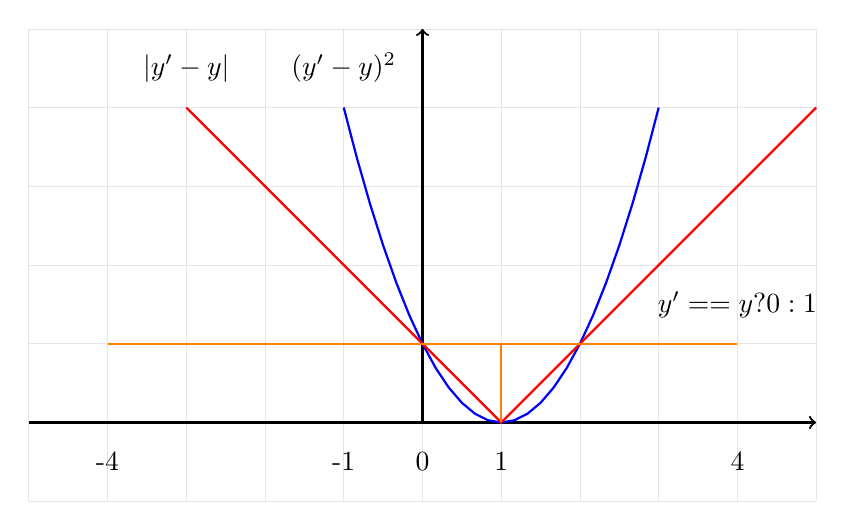
\begin{tikzpicture}
 \draw[help lines, gray!20] (-5,-1) grid (5,5);
 
 \foreach \x in {-4,-1,0,1,4}{
 	\node at (\x, -0.5) {\x};
 }
 
 \draw [->, thick] (-5,0) -- (0,0) -- (5,0);
 \draw [->, thick] (0,0) -- (0,5);
 
 \node at (-1,4.5) {$\cblue{(y' - y)^2}$}; 
 \node at (-3,4.5) {$\crouge{|y' - y|}$};
 \node at (4,1.5) {$\corange{y' == y ? 0 : 1}$};
 
 \draw [thick, blue, domain=-2:2] plot (\x +1, {\x * \x});
 \draw [thick, red, domain=-4:4]  plot (\x +1, {abs(\x)});
 
 \draw [-, thick, orange] (-4,1) -- (4,1);
 \draw [-, thick, orange] (1,1)  -- (1,0); 

\end{tikzpicture}
}

La formule orange nommé $Zero-one$ qui n'est pas convexe et qui est la première au quel on pense:
\formula{$f(y',y)\rightarrow y' == y ? 0 : 1$}

La formule rouge nommé $absolut$ qui est convexe mais trop punitif pour les petites erreurs:
\formula{$f(y',y) \rightarrow |y' - y|$}

La formule bleu nommé $quadratique$ qui est convexe et minimise les petits erreurs mais maximise les grosses erreurs:
\formula{$f(y',y) \rightarrow |y' - y|^2$}

\pagebreak
\section{Apprentissage par régression}

La régression est un problème de minimisation:\\

\begin{description}
\item[Paramètre]: Une fonction de mise à jour $f$
\item[Initialisation] $w_0 = 0$
\item[Pour toutes les entrées]:\begin{description}
\item[-] Recevoir l'observation $x_t$
\item[-] Faire une prédiction $y' = w_{t-1}^T x_i$
\item[-] Calculer la fonction de perte $(y',y)$
\item[-] Re apprendre le modèle en cas de mauvaise prédiction $w_t = f(w_{t-1})$
\end{description}
\end{description}

\subsection{Gradient Descent}

\begin{description}
\item[Initialisation] $w_0 = 0$
\item[Pour toutes les entrées]:\begin{description}
\item[-] Recevoir l'observation $x_t$
\item[-] Faire une prédiction $y' = w_{t-1}^T x_i$
\item[-] Calculer la fonction de perte $(y_t',y_t)^2$
\item[-] Re apprendre le modèle $w_t = w_{t-1} - \eta(y'_t-y_t) x_t$
\end{description}
\end{description}



\pagebreak
\section{Apprentissage par classification}

\pagebreak

